%===================================================================================
% PREÁMBULO
%-----------------------------------------------------------------------------------
\documentclass[a4paper,10pt]{article}

%===================================================================================
% Paquetes
%-----------------------------------------------------------------------------------
\usepackage{amsmath}
\usepackage{amsfonts}
\usepackage{amssymb}
\usepackage{jcematcom}
\usepackage[utf8]{inputenc}
\usepackage{listings}
\usepackage[pdftex]{hyperref}
\usepackage{array}

%-----------------------------------------------------------------------------------
% Configuración
%-----------------------------------------------------------------------------------
\hypersetup{colorlinks,%
	    citecolor=black,%
	    filecolor=black,%
	    linkcolor=black,%
	    urlcolor=blue}


%===================================================================================
% Presentacion
%-----------------------------------------------------------------------------------
% Título
%-----------------------------------------------------------------------------------
\title{Proyecto de Lógica Difusa. Simulación.}

%-----------------------------------------------------------------------------------
% Autores
%-----------------------------------------------------------------------------------
\author{\\
\name Antonio Jesús Otaño Barrera \email \href{mailto:a.otano@estudiantes.matcom.uh.cu}{a.otano@estudiantes.matcom.uh.cu}
	\\ \addr Grupo C411}


%===================================================================================
% DOCUMENTO
%-----------------------------------------------------------------------------------
\begin{document}

\maketitle

%===================================================================================
% Resumen y Abstract
%-----------------------------------------------------------------------------------
\selectlanguage{spanish} % Para producir el documento en Español


%===================================================================================


\section{Características del sistema de inferencia propuesto}\label{sec:0}
%---------------------------------------------------------------------------------------------------------------------------------------------------------------------

  \paragraph{} El sistema de inferencia propuesto acepta reglas con  múltiples variables de entrada y múltiples variables de salida. Las variables
  en la entrada pueden ser tanto valores (singleton) como conjuntos difusos. El sistema permite trabajar con funciones de membresía triangulares,
  trapezoidales, singleton, y rectas. Los métodos de inferencia que tiene implementados son los de Mamdani y Larsen, y los métodos de desdifusificación que
  brinda son los de Centroide (Center of Area), Bisección (Bisector of Area), y Media de los Máximos (Mean of Maximum).

%===================================================================================

\section{Principales ideas seguidas para la implementación del sistema}\label{sec:1}
%---------------------------------------------------------------------------------------------------------------------------------------------------------------------

	\paragraph{} El sistema fue implementado en Python y consiste en una librería que permite a cualquier otro programador usarla para
	resolver (siempre y cuando esté bien modelado) cualquier problema cuya solución se obtenga mediante inferencia difusa. El programador
	puede escoger el método de inferencia y el método de desdifusificación que más se ajuste al problema con que está tratando. Dado que el dominio de las variables 			linguísticas puede ser un conjunto continuo es necesario particionar el mismo en un número finito de segmentos o niveles para poder llevar a cabo los métodos de 				inferencia y desdifusificación. La discretización que se realiza es uniforme sobre todo el dominio  y es tarea del programador definir el número de segmentos o niveles en 		que se divide el mismo.  La implementación del sistema utiliza  cuatro entidades	fundamentales: conjuntos difusos, variables  linguísticas, reglas difusas y bases de reglas 		difusas. Las variables linguísticas son representadas con un dominio y un conjunto de términos en forma de conjuntos difusos cuyo dominio es el mismo que el de la 			variable y cuya función de membresía es decidida por el programador entre los posibles tipos explicados en la sección \ref{sec:0}. Por otro lado, las reglas difusas constan 		de un antecedente y un consequente; cada uno es una lista de pares (variable, término). Las bases de reglas difusas guardan un conjunto de reglas difusas, que sólo son 		de tipo MISO (múltiples entradas y una única salida). Para manejar las variables de tipo MIMO (múltiples entradas y múltiples salidas) se procede convirtiéndolas en 			múltiples reglas de tipo MISO, una por cada variable de control. Los métodos de agregación reciben como entrada una lista de conjuntos difusos que representan los 			valores que toman las variables de estado y devuelven una lista de conjuntos difusos que representan a las variables de control. Si la entrada consiste de valores simples 		entonces es necesario convertirla en conjuntos difusos de tipo singleton. A manera de ejemplo, si la entrada es el valor puntual $x_{0}$ entonces necesita ser 					transformado como se muestra en la figura \ref{fig:fuzzification}:
	
	\begin{figure}[h]
		\begin{center}		
			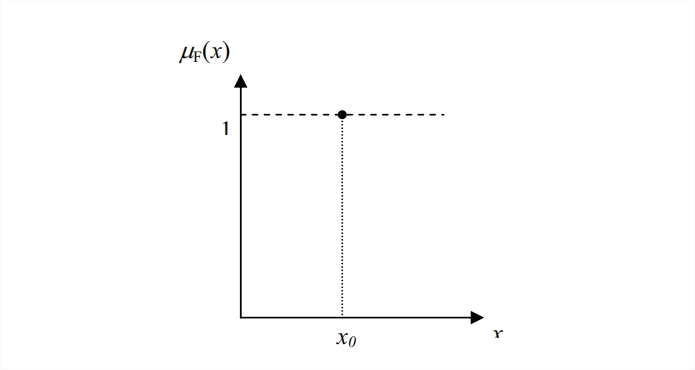
\includegraphics[width=200px, height=200px]{images/fuzzification.jpg}
		\end{center}
		\caption{Método de fusificación.\label{fig:fuzzification}}%
	\end{figure}
	
	Los métodos de desdifusificación se encargan de convertir los conjuntos difusos que devuuelven los métodos de agregación en valores puntuales. Como se dijo en la sección \ref{sec:0} hay tres variantes de desdifusificación: Centroide, Bisección y Media de los máximos. En el caso del Método de Bisección, se utiliza el Método de los Trapecios como método de integración.
%===================================================================================

\section{Propuesta de problema a solucionar mediante inferencia difusa}\label{sec:3}
%---------------------------------------------------------------------------------------------------------------------------------------------------------------------

  \paragraph{}   El problema propuesto consiste en simular el movimiento de un robot sobre un pasillo en el que existen obstáculos.
  El robot tiene sensores que le permiten detectar la distancia a la que se encuentra del objeto más cercano así como el ángulo que forma
  con el mismo. Conocidos estos parámetros el robot debe determinar que dirección tomar para evitar chocar con el obstáculo. Las siguientes reglas definen en detalle el 		  problema.
	\begin{enumerate}
	\item{La distancia se mide en metros y los ángulos en grados sexagesimales}
	\item{Los obstáculos tienen forma rectangular y sus lados varian entre 5 y 10 metros}
	\item{El robot es un punto en el espacio que se desplaza un metro de distancia por cada unidad de tiempo}
	\item{El pasillo constituye un rectángulo de ancho 60 y alto 100}
	\item{El robot concluye existosamente su tarea si llega al final del pasillo sin chocar con ningún obstáculo}
	\item{Las paredes del pasillo también constituyen obstáculos}
	\item{El robot comienza en la posición (30, 0)}
	\item{Los obstáculos están situados aleatoriamente en los últimos 70 metros del pasillo}
	\item{El total de objetos en el pasillo siempre será 5}
	\item{Para medir la distancia y el ángulo con respecto al obstáculo tomamos como referencia el punto más cercano del obstáculo al robot (Figura \ref{fig:distance_angle})}
	\end{enumerate}
	 
	 \begin{figure}[h]
		\begin{center}
			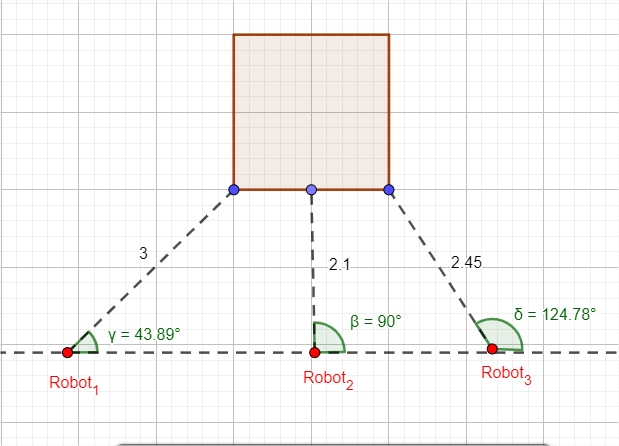
\includegraphics[width=200px, height=200px]{images/distance_angle.jpg}
		\end{center}
		\caption{Ejemplos de cómo se determina la distancia y el ángulo respecto a un obstáculo \label{fig:distance_angle}}%
	\end{figure}

\subsection{Variables linguísticas definidas}\label{sub:variables}
\paragraph{}A partir del enunciado anterior podemos definir tres variables lingüisticas que nos permitirán modelar el problema, como se muestra en la Tabla \ref{tab:lv}.




\subsection{Selección de las funciones de membresía}\label{sub:membership_functions}
	\paragraph{} En las figuras \ref{fig:distance_plot}, \ref{fig:angle_plot} y \ref{fig:direction_plot} se muestran las funciones de membresía asignadas a los términos de las variables Distancia, Ángulo y Dirección respectivamente.
	   
	\begin{figure}[p]
		\begin{center}
			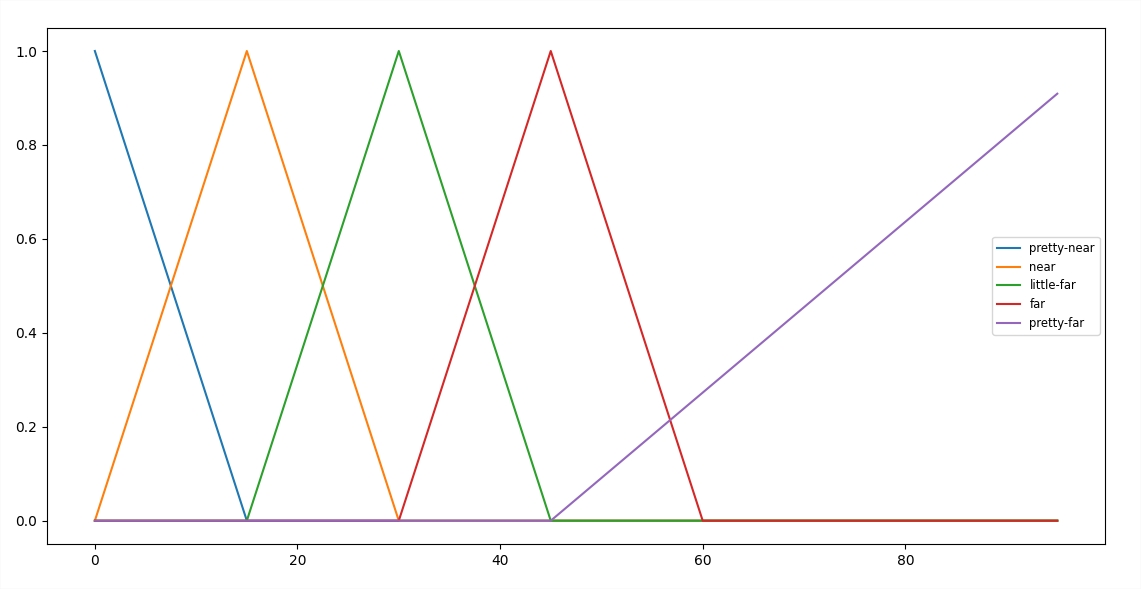
\includegraphics[width=400px, height=200px]{images/distance_plot.jpg}
		\end{center}
		\caption{Distancia \label{fig:distance_plot}}%
	\end{figure}	
	\begin{figure}[p]
		\begin{center}
			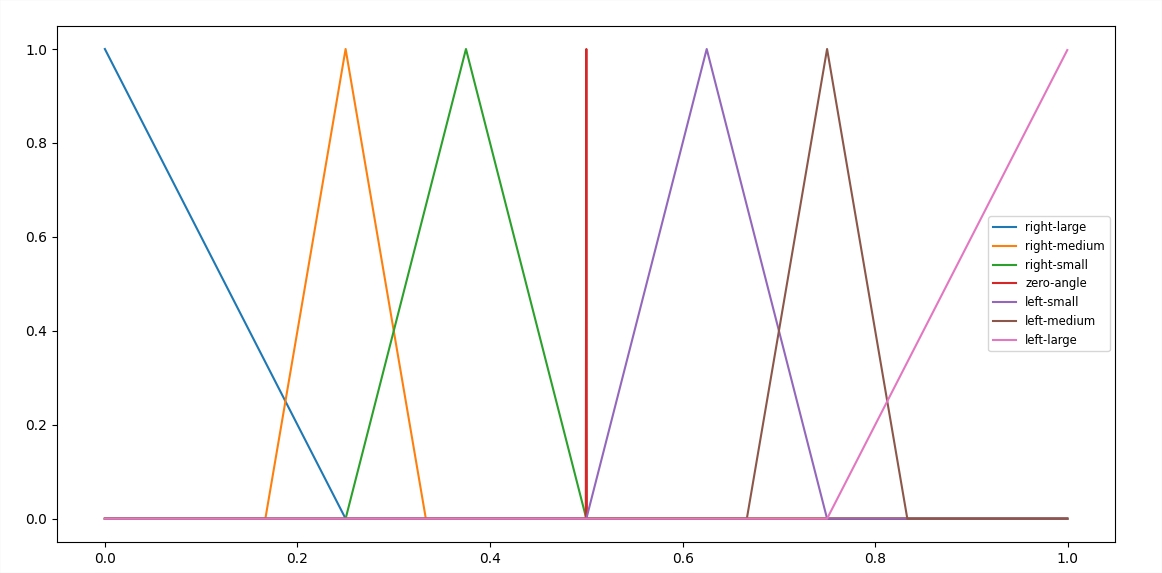
\includegraphics[width=400px, height=200px]{images/angle_plot.jpg}
		\end{center}
		\caption{Ángulo \label{fig:angle_plot}}%
	\end{figure}	
	\begin{figure}[p]
		\begin{center}
			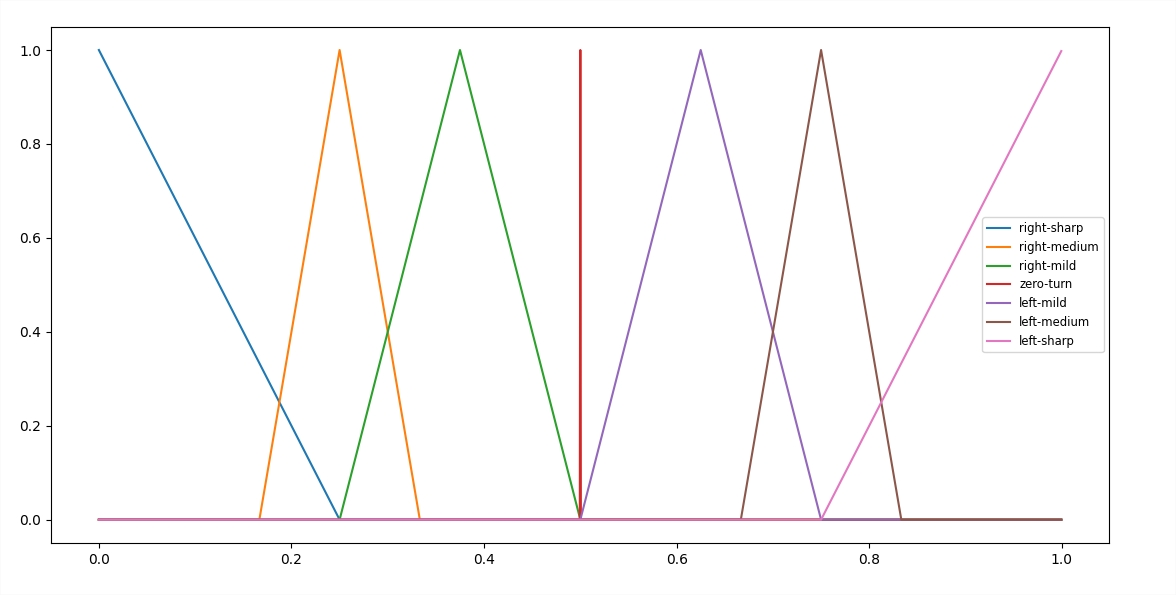
\includegraphics[width=400px, height=200px]{images/direction_plot.jpg}
		\end{center}
		\caption{Dirección \label{fig:direction_plot}}%
	\end{figure}
	
	
\begin{table}
	\begin{center}
		 \begin{tabular}{| c | c | c |p{3.5cm}|}
			  \hline
			    Variable & Tipo & Dominio & Términos  \\ \hline
			    Distancia & Estado & [0, 100] & muy cerca (PN), \newline cerca (N), \newline un poco lejos (LF), \newline lejos (F), \newline muy lejos (PF)  \\ \hline
			    Ángulo & Estado & [0, 180] & der-grande (RL), \newline der-mediano (RM), \newline der-pequeño (RS), \newline nulo (Z), \newline izq-pequeño (LS), \newline 					izq-mediano (LM), \newline izq-grande (LL)  \\ \hline
			    Dirección & Control & [0, 180] & izq-cerrado (LS), \newline izq-moderado (LME), \newline izq-leve (LMI), \newline recto (ZT), \newline der-leve (RMI), \newline 				der-moderado (RME), \newline der-cerrado (RS) \\ \hline
		  \end{tabular}		  
		  \caption{Variables lingüisticas del problema  \label{tab:lv}}%		 
	\end{center}
\end{table}

\subsection{Construccion de la base de reglas difusas}\label{sub:fuzzy_rule_base}
	\paragraph{} Para representar el conocimiento  utilizamos reglas difusas de la forma:
	
	\begin{quote}
		``Si la distancia es $A_{i}$ y el ángulo es $B_{i}$, entonces la direccion es $C_{i}$.''
	\end{quote}
	
		A partir de un análisis detallado del problema se pudo construir el conjunto de reglas difusas representado en la Figura \ref{fig:rules}.
	Para leer una regla escogemos una fila para la distancia y una columna para el ángulo y la intersección es la dirección. Por ejemplo, si la distancia es cerca(N) y el ángulo 		es pequeño a la derecha (RS) entonces la direccion que debemos tomar es doblando a la izquierda cerrado (LS). 
	
	\begin{figure}[!h]
		\begin{center}
			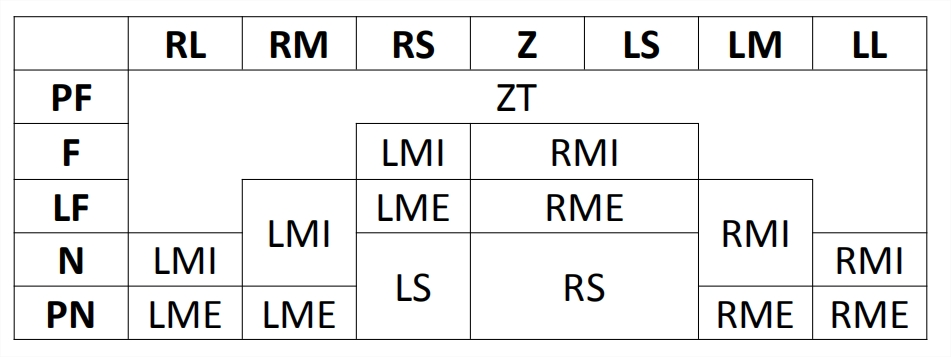
\includegraphics[width=250px, height=200px]{images/rules.jpg}
		\end{center}
		\caption{Base de reglas difusas \label{fig:rules}}
	\end{figure}
	
	
\section{Consideraciones obtenidas a partir de la solución del problema con el sistema de inferencia implementado}\label{sec:4}	

	Fue necesario encontrar un número adecuado de segmentos en los que dividir el dominio de las variables para obtener un balance entre calidad y rapidez. Los mejores parámetros encontrados fueron de 20 para la distancia y 30 para la dirección y el ángulo. El método de desdifusificación de Media de los Máximos fue descartado desde el comienzo al no brindar resultados satisfactorios. Se realizaron un total de 30 simulaciones con las combinaciones de Larsen y Centroide, Larsen y Bisección, Mamdani y Centroide y Mamdani y Centroide, pasando todas las pruebas con éxito.


\section{Sobre la estructura del proyecto}\label{sec:5}
	La implementación consta de dos partes:
	\begin{enumerate}
	\item{La implementación del sistema de inferencia, localizada en el directorio \emph{/src/fis}. La misma consta de los siguientes módulos:
	\begin{description}
		\item[classes.py] Definición de las clases que representan las variables linguísticas, conjuntos difusos, reglas y bases de reglas difusas.
		\item[defuzzification.py] Métodos de desfusificación (Centroide, Bisección y Media de los Máximos)
		\item[fuzzy\_inference\_system.py] Provee la interfaz necesaria para trabajar con el sistema de inferencia difusa.
		\item[inference\_methods.py] Métodos de inferencia (Mamdani y Larsen).
		\item[membership\_functions.py] Implementación de funciones de membresía (triangular, trapezoidal, singleton, recta)	 
	\end{description}}
	\item{La solución del problema propuesto, localizada en \emph{/src}. A su vez consta de 3 módulos:
	\begin{description}
		\item[main.py] Interfaz de usuario que permite evaluar el sistema de inferencia difusa a través del problema propuesto. El usuario provee los parámetros de distancia y ángulo y obtiene la correspondiente dirección.
		\item[simulation.py] Encargado de realizar las simulaciones.
		\item[robot\_motion.py] Modelación del problema usando el sistema de inferencia propuesto.
	\end{description}}
	\end{enumerate}	


\label{end}


\end{document}
